% Challenges (tokenization, conditional generation, attention, data cleaning), training of the model)
Adapting the transformer architecture — originally developed for text processing — to symbolic music presents many challenges.
Symbolic music datasets, unlike text corpus, are limited in both size and diversity, posing challenges for training robust models\cite{le_natural_2024}.
Tokenization must be tailored to represent pitch, duration, and dynamics, while attention mechanisms require adaptation to capture the hierarchical and temporal structure of music.
Finally, data cleaning and preprocessing steps are critical to standardize music scores and ensure the compatibility with sequence models.

% State of the art (survey, DadaGP, Compound Gen, Structure-informed positional encoding, gen coherent drum accompaniment)
% ResearchRabbit to find potential other articles

\subsection{Data availability}


Symbolic music datasets are a cornerstone for training deep learning models, yet their availability and quality significantly vary across domains.
In music composition and generation, datasets are often limited in size and diversity, especially when compared to text or image datasets.
For bass guitar tablatures, the challenge is even more pronounced due to the niche nature of the instrument and the focus on other instruments in existing datasets.


The MIDI standard has dominated symbolic music datasets for decades, allowing the development of resources like the Lakh MIDI dataset and MAESTRO dataset.
However, while these datasets offer general-purpose symbolic music, they lack the specificity required for tasks involving tablatures or instrument-specific representation.
The GuitarSet dataset, for example, focuses on acoustic guitar transcription but does not provide sufficient symbolic information for bass guitar.
Similarly, the DadaGP dataset addresses the need for multi-instrument symbolic music data in tablature format, but its emphasis is on rock and metal genres, which limits the diversity of bass guitar styles\cite{sarmento_dadagp_2021}.


Bass guitar data, especially in tablature format, suffers from a lack of standardization and availability.
Tablature files are often stored in private formats like GuitarPro or as non-standardized text files, making it challenging to preprocess them for machine learning tasks\cite{sarmento_dadagp_2021}.
Moreover, rhythm and dynamics, critical elements in bass guitar playing, are frequently absent in publicly available tablatures, complicating their utility in generative tasks.


Efforts like DadaGP illustrate the potential of GuitarPro files repositoriess to create symbolic datasets that include bass guitar parts.
Moreover DadaGP also provides a tokenized format inspired by MIDI encodings, offering a foundation for training sequence models.
On the other hand, pre-trained models on broader datasets like MAESTRO or Lakh MIDI can be fine-tuned on smaller datasets, reducing the dependency on large volumes of task-specific data\cite{makris_conditional_2022, sarmento_dadagp_2021}.
For our project, we use the DadaGP dataset. Its very specific tokenization will be discussed in the next section.


\subsection{Tokenization}

Tokenization in the context of deep learning music generation has been discussed by several previous works\cite{agarwal_structure-informed_2024, makris_conditional_2022, sarmento_dadagp_2021, hsiao_compound_2021, cournut_encodages_2020}.

% General overview of the possible startegies (NLP survey)
Tokenization in music involves converting complex musical content into a sequence of elements that can be processed computationally.
Much like tokenization in natural language processing (NLP), it breaks down music into manageable units, though in music, the focus is on musical features like pitch, duration, and velocity.
In symbolic music information retrieval (MIR), tokenization strategies are generally classified into two categories: time-slice-based and event-based. 
Time-slice-based tokenization divides music into fixed-time intervals, such as 16th notes, which can be represented in formats like piano rolls or multi-hot vectors, capturing simultaneous notes at each time slice.
Event-based tokenization, on the other hand, focuses on specific musical events, such as a note being played or a measure starting, often using formats like MIDI, which encode music as a series of events.
This approach can involve elementary tokens, which represent individual features like pitch or duration, or composite tokens that aggregate multiple features into one token, providing a more compact representation.
Notably, tokenization strategies like REMI (Revamped MIDI-derived events) and MIDI-like tokenization allow for consistent representation of rhythmic and pitch elements while addressing complexities like polyphony and multiple tracks in multi-instrument music\cite{le_natural_2024, cournut_encodages_2020}.


% DadaGP tokenization
The DadaGP tokenization format adopts an event-based approach, similar to other music generation models, by representing musical events as discrete tokens.
It uses a Python script with PyGuitarPro to convert GuitarPro files into a tokenized sequence, beginning with metadata tokens such as artist, downtune, tempo, and start.
Pitched instrument notes are encoded with a combination of tokens representing instrument, note, string, and fret, while rests are denoted with a separate token structure.
For drumset sounds, a specific tokenization scheme using MIDI percussion maps is employed, where each drum sound is represented by a unique token (e.g., drums:note:36 for a kick drum).
The system also uses wait tokens to separate notes and rests, enabling the model to infer note durations without the need for explicit note-off tokens.
This approach ensures that new notes automatically silence previous ones, except in cases where ghost notes or let-ring effects are involved.
Additionally, the tokenization format records changes in musical structure, such as new measures, tempo shifts, and note effects, with each change being represented as a distinct token.
However, the tokenization does not encode dynamics or articulations. These are supposed to be inferred by the user after generation.


\begin{figure}[h!]
    \centering
    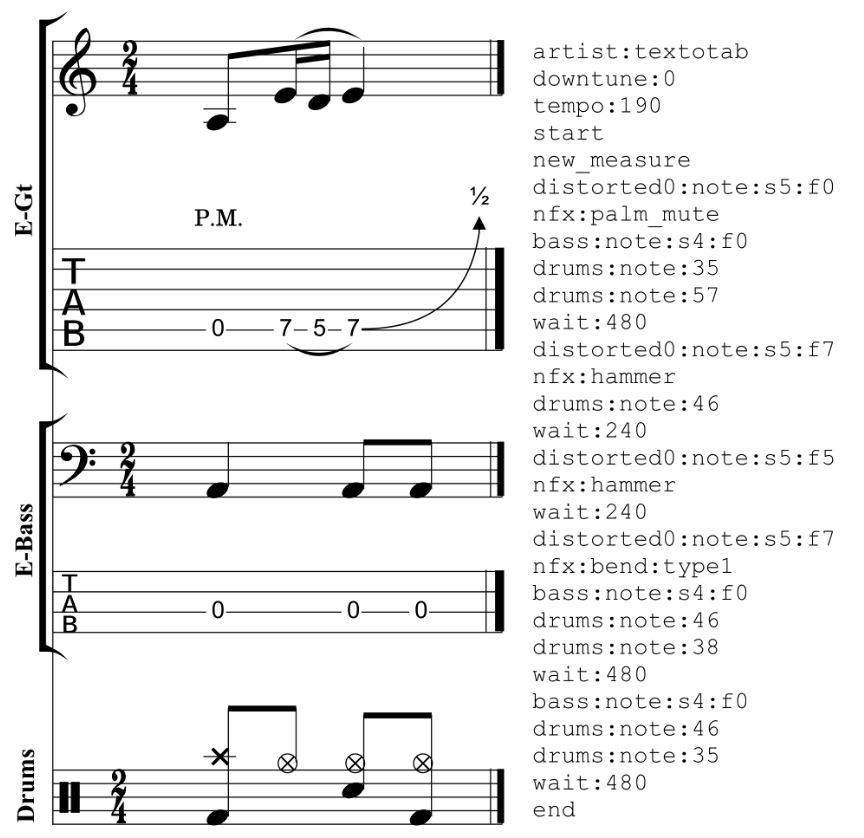
\includegraphics[width=.5\linewidth]{../images-figures/dadagp_tokenization_example_measure.png}
    \caption{Example measure with a distorted guitar, bass and drums in GuitarPro’s graphical user interface (left), and its conversion into token format (right). Figure taken from \cite{sarmento_dadagp_2021}}
    \label{fig:dadagp_tokenization}
\end{figure}


Figure \ref{fig:dadagp_tokenization} illustrates the tokenization process for a measure in a GuitarPro file, showing the conversion of a musical event into a tokenized sequence.
We notice the three first tokens are the metadata tokens. "start" token marks the beginning of the song.
Afterwards, each measure is announced by a "new\_measure" token.
In between, the instruments' notes are encoded using the tablature notation for the guitars.
For instance the first note played here is distorted0:note:s5:f0 (string 5, fret 0).
It is followed by a nfx token "nfx:palm\_mute", which is a note effect token that applies to the previous note.
Finally, the duration of the note is given by the wait token "wait:480" (480 ticks in GuitarPro correspond to an eighth note).
If no tokens of a specific instrument are present between two wait tokens, it means that the instrument keeps on playing the same note.
This is the case of the bass in the example.
Its first quarter note lasts for 960 ticks, therefore we have to look after the three first wait tokens (480 + 240 + 240) before seeing a new token for the bass.


% Compound Gen tokenization
As we plan to use the model built by Makris et al. in 2022, we will also consider the tokenization they used.
The proposed tokenization model introduces a compound word (CP) representation, inspired by previous CP-based approaches\cite{hsiao_compound_2021}.
Unlike traditional tokenization strategies such as MIDI-like or REMI, which encode music as a linear sequence of tokens, CP groups multiple features of a musical event into a single "super token" or "word".
This n-dimensional representation significantly reduces sequence length and improves computational efficiency in Transformer-based architectures\cite{makris_conditional_2022}.


In this model, the CP representation is adapted for an Encoder-Decoder architecture to condition drum generation on accompanying rhythm tracks, such as bass and guitar.
The Encoder processes a 5-dimensional CP representation that includes rhythm track features and high-level musical information like tempo and time signature, which are known to influence the complexity and density of drum tracks.
Both the Encoder and Decoder adopt bar-based segmentation, consistent with existing CP and REMI representations.
By combining rhythm section inputs and high-level parameters, this tokenization approach aligns with the fundamental musical principles of contemporary western music's rhythm section\cite{makris_conditional_2022}.
As said previously, our work will use the DadaGP tokenization. However, the nature of the generation task we want to perform is very similar to the one of Makris et al. in the sense that bass guitar and drums are part of the same rhythm section.


\begin{figure}[h!]
    \centering
    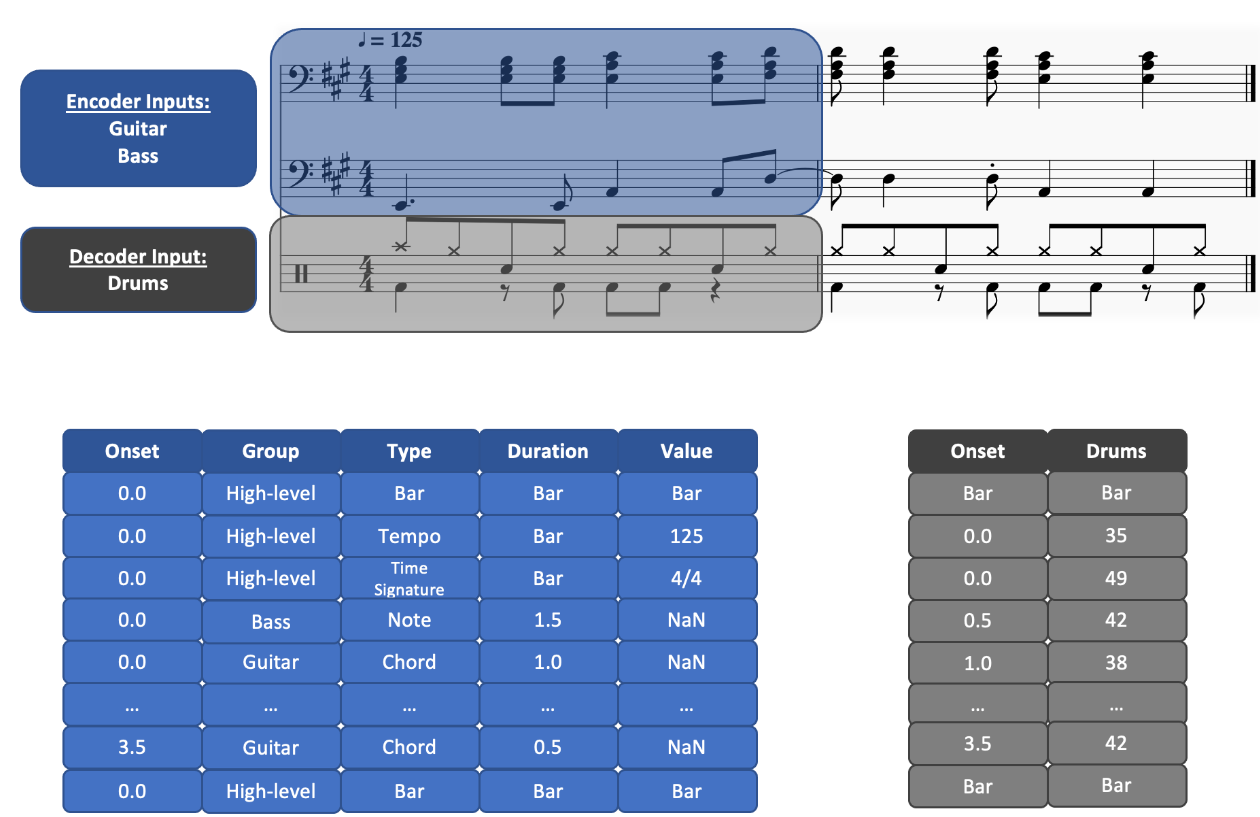
\includegraphics[width=.5\linewidth]{../images-figures/tokenization_makris.png}
    \caption{Example of a CP representation used for training. Figure taken from \cite{makris_conditional_2022}}
    \label{fig:compound_gen_tokenization}
\end{figure}


Figure \ref{fig:compound_gen_tokenization} shows an example of a CP representation used for training in the model developed by Makris et al.
We notice that the rhythmic section, composed of a rhythmic guitar and a bass (in blue on the figure), constitutes the conditioning part of the model.
Their representation as tokens encode the duration and type of the notes played, but not the pitch of the notes as it is not relevant for the drum generation task.
In grey, the drum part's encoding excludes all information about velocities and duration.
Drums notes and are only represented by their onset in the bar and the drum component played.

\subsection{Conditional generation models}

% Intro about conditional generation using control tokens (prompt tokens)
% --> GTR CTRL, ShredGP, ProgGP
Our first idea was to use the GuitarCTRL model developed by Sarmento et al. in 2021\cite{sarmento_gtr-ctrl_2023}.
The GTR CTRL model utilizes a Transformer-XL architecture\cite{dai_transformer-xl_2019}, which improves on the vanilla Transformer by introducing recurrence and modified positional encodings, enabling long-term dependency learning.
This model includes two key control types: instrumentation (inst-CTRL) and genre (genre-CTRL).
For instrumentation, tokens marking the start and end of each instrument are inserted into the header, guiding the model to generate music for specified instruments, such as bass and drums or distorted guitar and drums.
Genre control tokens are similarly placed at the beginning of the sequence, with a dataset covering over 200 songs per genre, including Metal, Rock, Punk, Folk, and Classical.
The model uses various prompts at inference, ranging from full-prompt (including two measures plus the genre token) to empty-prompt (only the genre token).
This model was used to generate a baseline result for our project, conditioning the generation to bass guitar only.


% Start with a historic of BI-LSTM in NLP (2015)
% Dive in makris et al model (BiLSTM) (SOTA in drum generation)
The model we wish to use for our project is the one developed by Makris et al. in 2022\cite{makris_conditional_2022}.
It employs an Encoder-Decoder architecture with a BiLSTM Encoder and a Transformer Decoder utilizing Relative Global Attention.
The Encoder is made of several BiLSTM layers. It processes Compound Representation (CP) inputs to generate a latent variable z that encodes high-level features of the input and conditional tracks.
BiLSTM (Bidirectional Long Short-Term Memory) were first introduced by Graves et al. in 2005\cite{graves_framewise_2005}. It is a type of recurrent neural network (RNN) that processes data in both forward and backward directions.
This allows the model to consider both past (previous time steps) and future (upcoming time steps) context in the sequence
The Decoder consists of self-attention layers and feed-forward layers. 
It combines z with previous timestep embeddings to predict drum onsets and pitches.



The model uses input sizes that are different from the ones we may use with our tokenization.
However we are interested in the ability of the model to generate conditionnally throughout the whole sequence.
In comparison, GTR CTRL only conditions the generation at the beginning of the sequence.
One of the issue we encountered when generating bass guitar was that other instruments ended up being generated further in the sequence.
To avoid this we tried setting the probability of predicting tokens from any other instruments to 0, but even then the bass lines generated were not coherent.
This model is simply not suited for our task which explains our motivations to adapt the BiLSTM model.
